\documentclass{article}      % Specifies the document class

\usepackage{amsmath}
\usepackage{algpseudocode}
\usepackage{algorithm}
\usepackage{forloop}
\usepackage{graphicx}


\newcounter{ct}
\newcommand{\markdent}[1]{\forloop{ct}{0}{\value{ct} < #1}{\hspace{\algorithmicindent}}}
\newcommand{\markcomment}[1]{\Statex\markdent{#1}}

\algnewcommand\algorithmicforeach{\textbf{for each}}
\algdef{S}[FOR]{ForEach}[1]{\algorithmicforeach\ #1\ \algorithmicdo}

\begin{document}
 \large Intro about re project \\
 \large BDD Modeling Process \\
\begin{figure}
  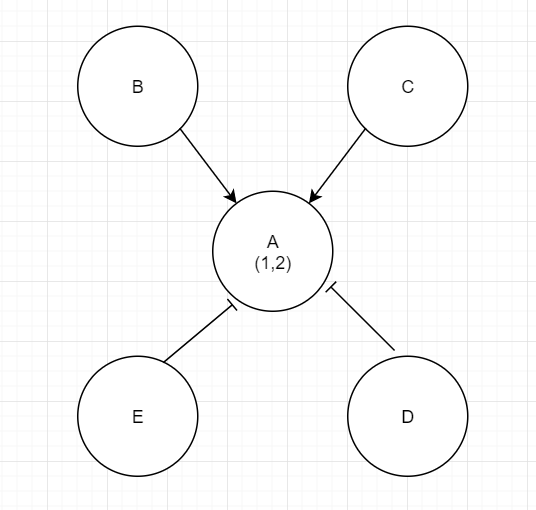
\includegraphics[ext=.png type=png width=0.2]{ex1.png}
  \caption{A boat.}
  \label{fig:boat1}
\end{figure}

\begin{algorithm} \caption{Process Experiments List}
\begin{algorithmic}[1]
\Function {ProcessExperiments}{}
\State $list \gets \text{list of experiments}$
\State $booleanNetwork \gets \text{boolean network graph and functions}$
\State \textbf{begin function}
    \ForEach {$e_1$, $e_2$ pair of experiments in list}
        \State $res \gets FindValidMerges(e_1, e_2, bn)$
        \State $newList \gets \text{a copy of experiments list}$
        \State \text{add res to top of the list (can be multiple)}
        \State \text{call} $ProcessExperiments(newList, booleanNetwork)$
        \Comment{Backtracking process}
    \EndFor
\EndFunction
\State \Comment{Missing part: how the algorithm finish}
\end{algorithmic}
\end{algorithm}
\begin{algorithm}
\begin{algorithmic}[1]
\Function {FindValidMerges}{}
\State $exp1 \gets \text{first experiment}$
\State $exp2 \gets \text{second experiment}$
\State $booleanNetwork \gets \text{boolean network graph and functions}$
\State \textbf{begin function}
    \ForEach {s state in exp1}
        \State $mergedExperiment \gets \text{connect s with begin of exp2}$
        \If{\text{IsValidMerge(mergedExperiment, booleanNetwork)}}
                \State \text{add mergedExperiment to returnList }
        \EndIf
    \EndFor
    \ForEach {s state in exp2}
        \State $mergedExperiment \gets \text{connect s with begin of exp1}$
        \If{IsValidMerge(mergedExperiment, booleanNetwork)}
                \State \text{add mergedExperiment to returnList }
        \EndIf
    \EndFor
\EndFunction
\end{algorithmic}
\end{algorithm}
\begin{algorithm}
\begin{algorithmic}[1]
\Function {IsValidMerge}{}
\State $exp \gets \text{an experiment}$
\State $booleanNetwork \gets \text{boolean network graph and functions}$
\State $bdd \gets \text{an new empty BDD}$
\State \text{Add states values to BDD}
\State $BDD \gets \text{an empty BDD}$
\State \textbf{begin function}
    \ForEach {\text{s state in experiment}}
        \State $BDD \gets \text {BDD AND s}$
    \EndFor
\State $functionBDD \gets \text{an empty BDD}$
    \ForEach {\text{v vertex in booleanNetwork}}
        \State $incomeEdges \gets \text{income edges to vertex v}$
        \State $availableFunctions \gets \text{available functions for vertex v}$
        \State $functionBDD \gets \text{functionBDD AND CreateFunctionRepresentation(v, availableFunctions, incomeEdges, experiment.length)}$
    \EndFor
\State $BDD \gets \text{BDD AND functionBDD}$
\State $BDD \gets \text{BDD AND 1}$
\If{BDD is Empty}
    \State \text{return false}
\EndIf
    \State \text{return true}
\EndFunction
\end{algorithmic}
\end{algorithm}
\begin{algorithm}
\begin{algorithmic}[1]
\Function {CreateFunctionRepresentation}{}
\State $availableFunctions \gets \text{list of possible functions}$
\State $letter \gets \text{current letter}$
\State $edges \gets \text{list of edges letter}$
\State $length \gets \text{experiment length}$
\State \textbf{begin function}
\State $functionBDD \gets \text{an empty BDD}$
    \For{\texttt{i=0;i<length;i++}}
        \State $tempBDD \gets \text{an empty BDD}$
        \ForEach {\text{F function in availableFunctions}}
            \State $tempBDD \gets \text{tempBDD OR ($f_i$ and $F_i$implementation(edges))}$
            \State \Comment{Missing part: optional parameters}
        \EndFor
        \State $tempBDD \gets \text{tempBDD AND (f1, f2, .., fn}$
        \State \Comment{ensure one of the function has been choosen}
        \State $functionBDD \gets \text{functionBDD AND $letter_{i+1}$ equal tempBDD}$
    \EndFor
    \State \text{return functionBDD}
\EndFunction
\end{algorithmic}
\end{algorithm}

\end{document}